\documentclass[12pt,a4paper]{article}
\title{%
  Øving 1 \\
  \large IELET1002 - Datateknikk \\
  }
\author{Gunnar Myhre, BIELEKTRO}

\usepackage{graphicx}
\usepackage[utf8]{inputenc}
\usepackage[norsk]{babel}
\usepackage{pgfplots}
\graphicspath{ {./images} }

\setlength\parindent{0pt}

\begin{document}
  \maketitle
  \section{Oppgåve 1}
    \subsection{a)}
      \begin{center}
        \begin{tabular}{ |c|c|c|c| }
          \hline
          Binær & Oktal & Hexadecimal & Decimal \\
          \hline
          101101011 & $\backslash553$ & 0x16B & 363 \\
          \hline
          11001101  & $\backslash315$ & 0xCD  & 205 \\
          \hline
          10111010001111  & $\backslash27217$ & 0x2E8F  & 11919 \\
          \hline
          101100111001  & $\backslash5471$  & 0xB39 & 2873 \\
          \hline
          0,10011 & $\backslash0,46$  & 0x0,98  & 0,59375 \\
          \hline
        \end{tabular}
      \end{center}

      Utrekning på neste side

      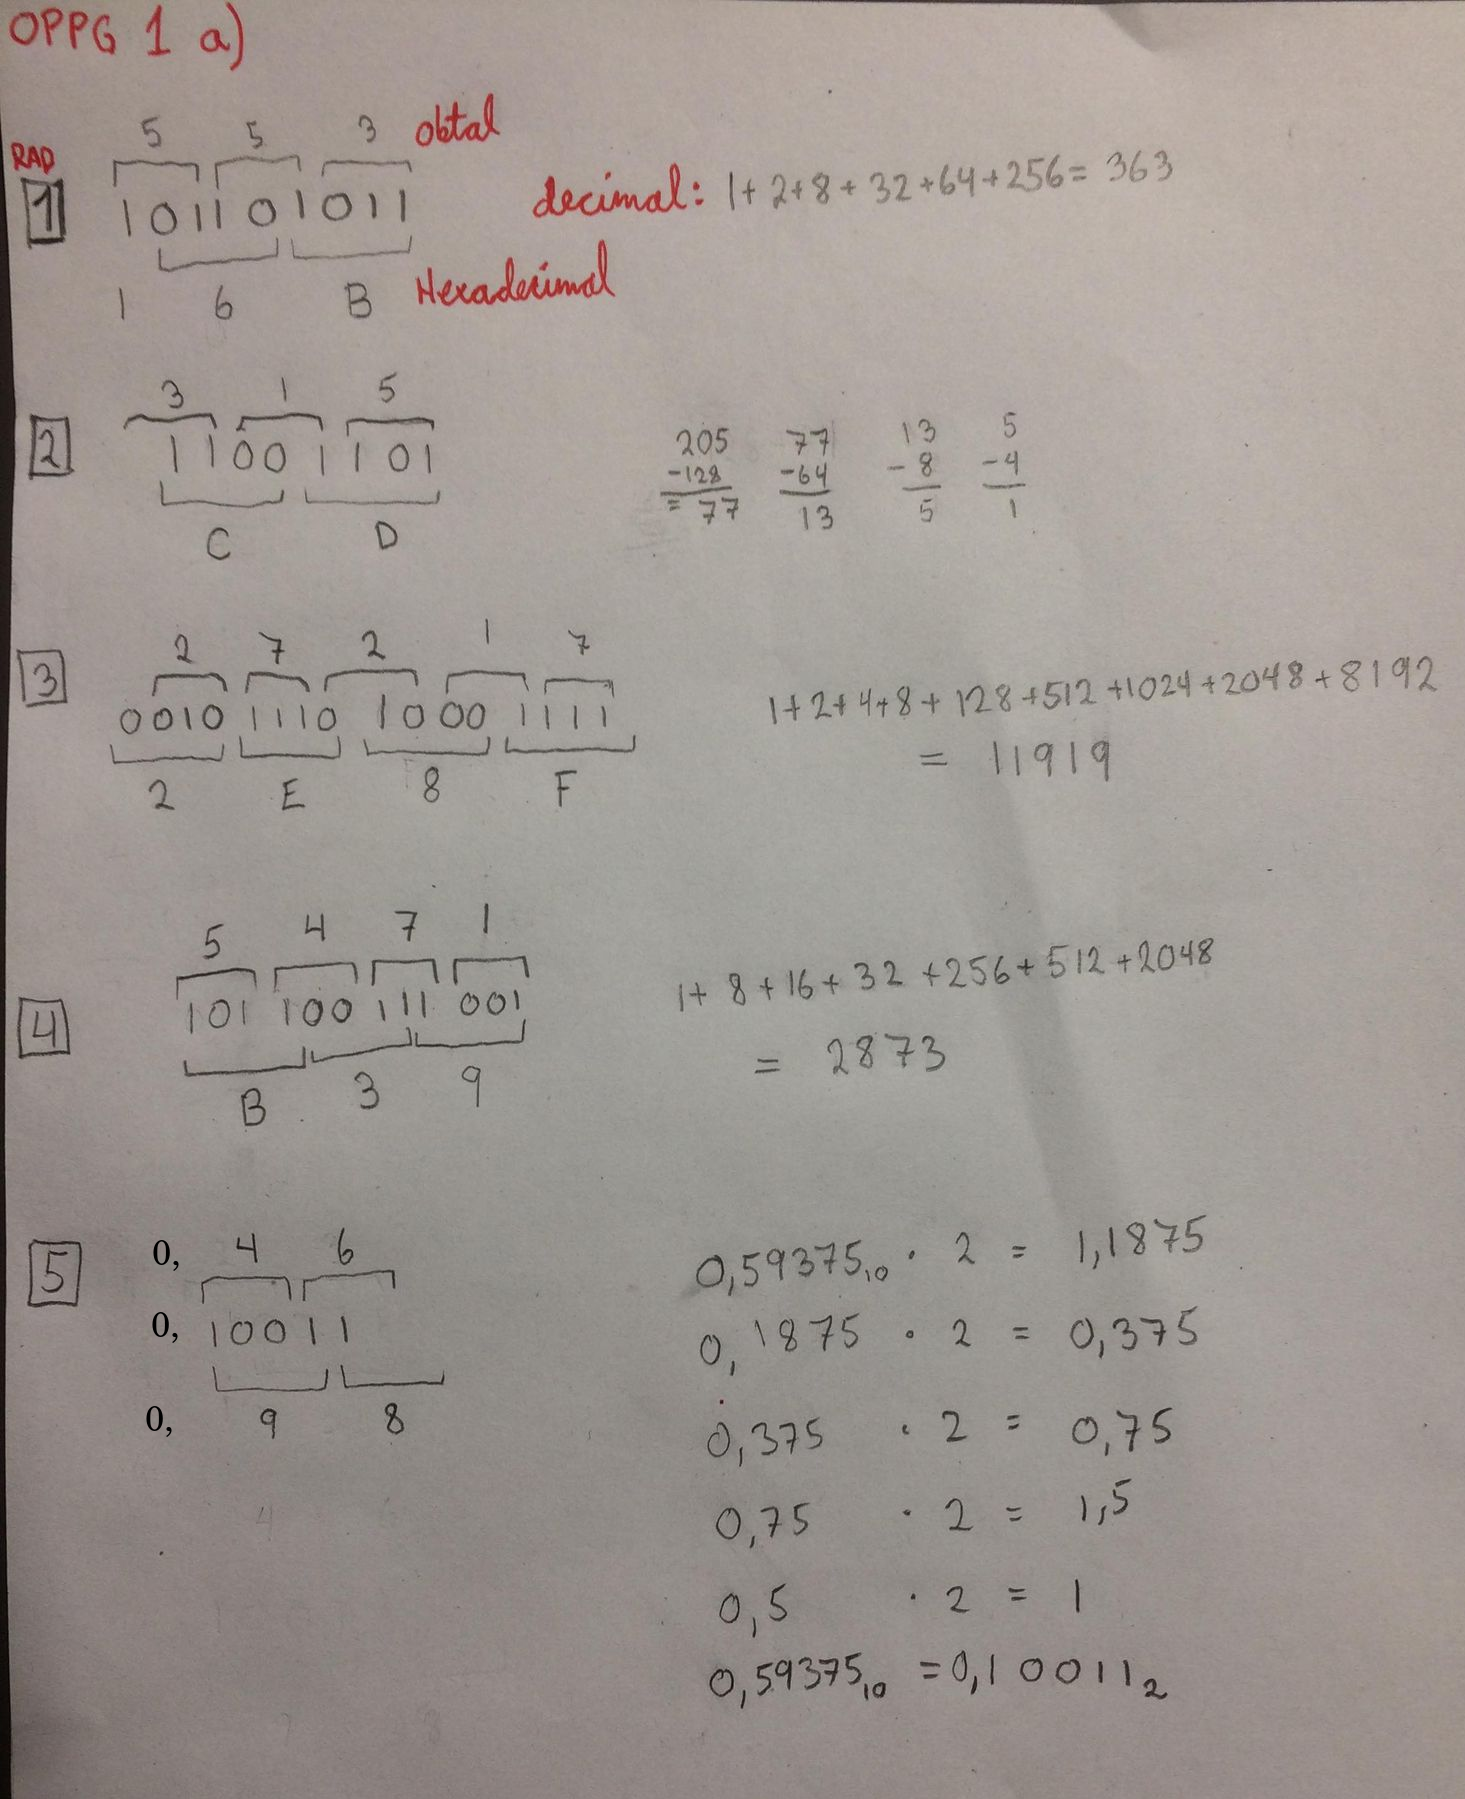
\includegraphics[width=\textwidth]{01_1_a}
      \newpage

  \section{Oppgåve 2}
    \begin{centering}
    $0,7_{10} \cdot 2 = 1,4$ \\
    $0,4_{10} \cdot 2 = 0,8$ \\
    $0,8_{10} \cdot 2 = 1,6$ \\
    $0,6_{10} \cdot 2 = 1,2$ \\
    $0,2_{10} \cdot 2 = 0,4$ \\
    $0,4_{10} \cdot 2 = 0,8$ \\
    $0,8_{10} \cdot 2 = 1,6$ \\
    $0,6_{10} \cdot 2 = 1,2$ \\
    $0,2_{10} \cdot 2 = 0,4$ \\
    $0,4_{10} \cdot 2 = 0,8$ \\
    \end{centering}

    Her får vi $0,7_{10}=0,10110011001100_{2}$. . . der $1100$ vil gjenta
    seg for alltid, divisjonen vil med andre ord aldri gå opp og gjeve
    oss 0 i rest. \\

    $1 \cdot \frac{1}{2} = 0,5 \rightarrow sum = 0,5$ \\
    $0 \cdot \frac{1}{4} = 0$ \\
    $1 \cdot \frac{1}{8} = 0,125 \rightarrow sum = 0,625$ \\
    $1 \cdot \frac{1}{16} = 0,0625 \rightarrow sum = 0,6875$ \\
    $0 \cdot \frac{1}{32} = 0$ \\
    $0 \cdot \frac{1}{64} = 0$ \\
    $1 \cdot \frac{1}{128} = 0,0078125 \rightarrow sum = 0,6953125$ \\
    $1 \cdot \frac{1}{256} = 0,00390625 \rightarrow sum = 0,69921875$ \\
    $0 \cdot \frac{1}{512} = 0$ \\
    $0 \cdot \frac{1}{1024} = 0$ \\
    $1 \cdot \frac{1}{2048} = 0,000488281 \rightarrow sum = 0,699707031$ \\
    $1 \cdot \frac{1}{4096} = 0,000244141 \rightarrow sum = 0,699951172$ \\
    $0 \cdot \frac{1}{8192} = 0$ \\
    $0 \cdot \frac{1}{16384} = 0$ \\

    Som venta vil talet konvergere mot $0,7$ for fleire bit bak fraksjonsteiknet.
    I dette tilfellet er 8 bit bak fraksjonsteiknet nok til å gjeve oss mindre
    enn $1\%$ feil.
    
    
  \section{Oppgåve 3}
    Utfører addisjonane med 2-komplementsreprentasjon \\
    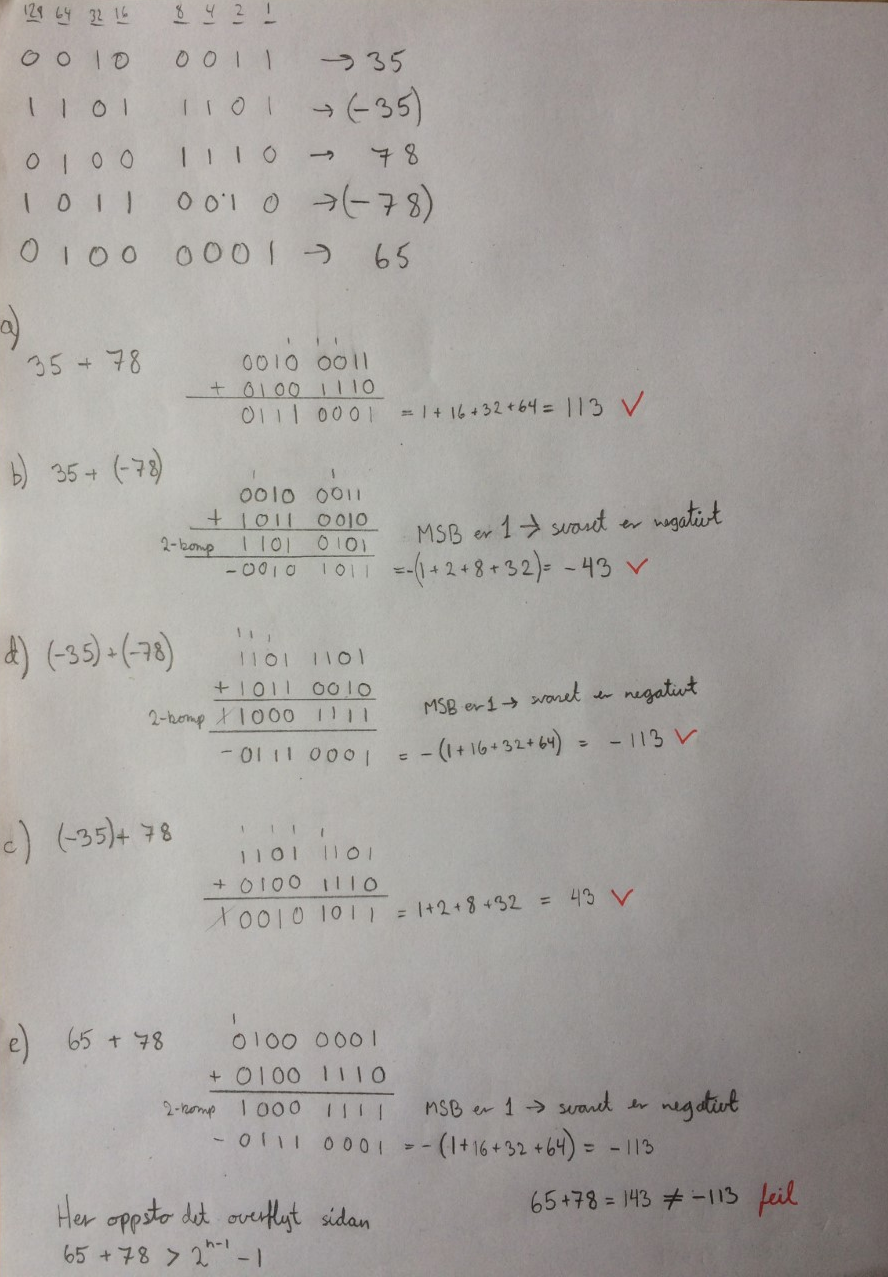
\includegraphics[width=\textwidth]{01_3.png}
  
  \section{Oppgåve 4}
    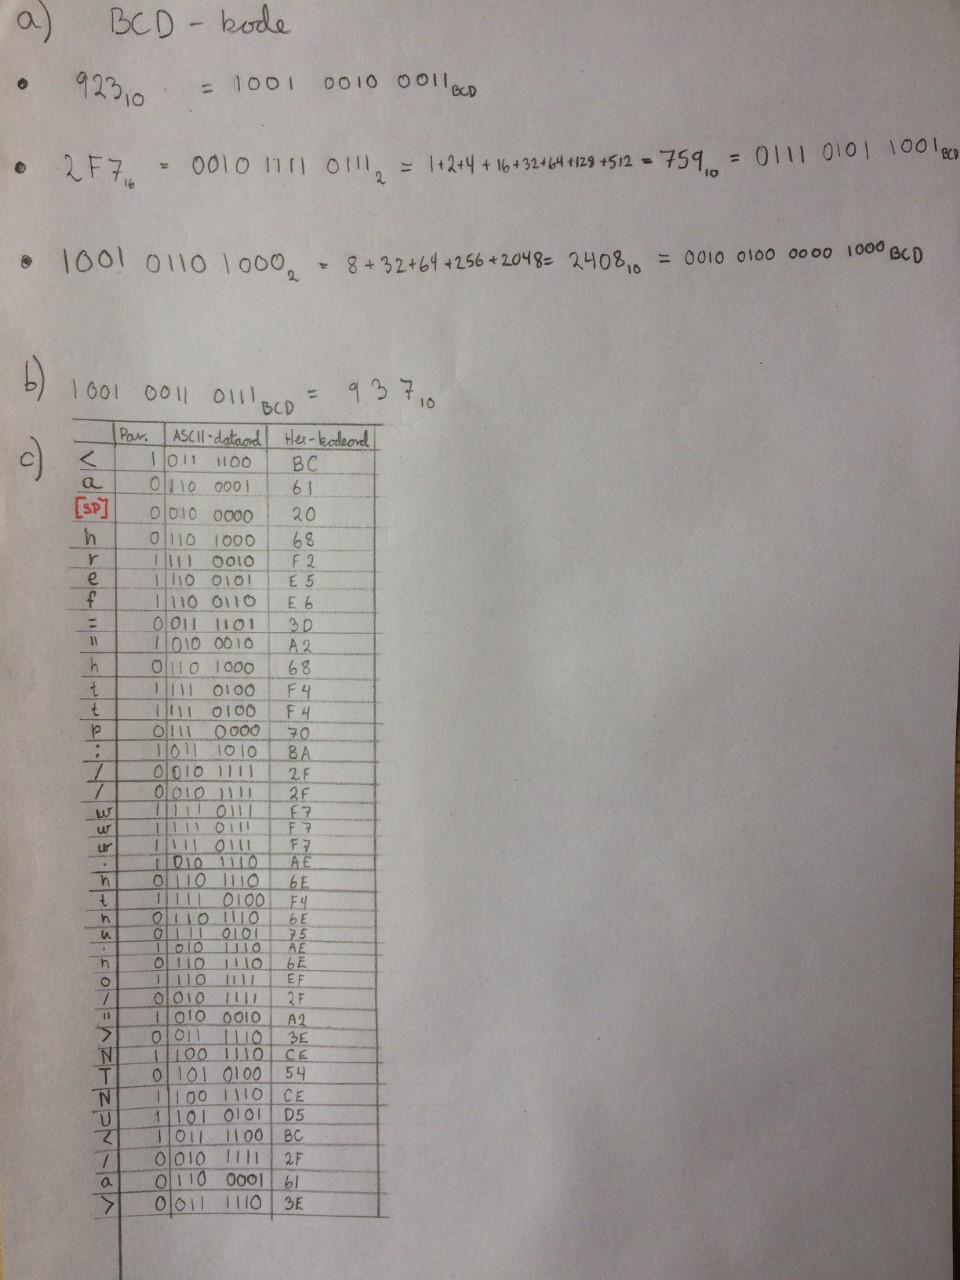
\includegraphics[width=\textwidth]{01_4.png}

  \section{Oppgåve 5}
    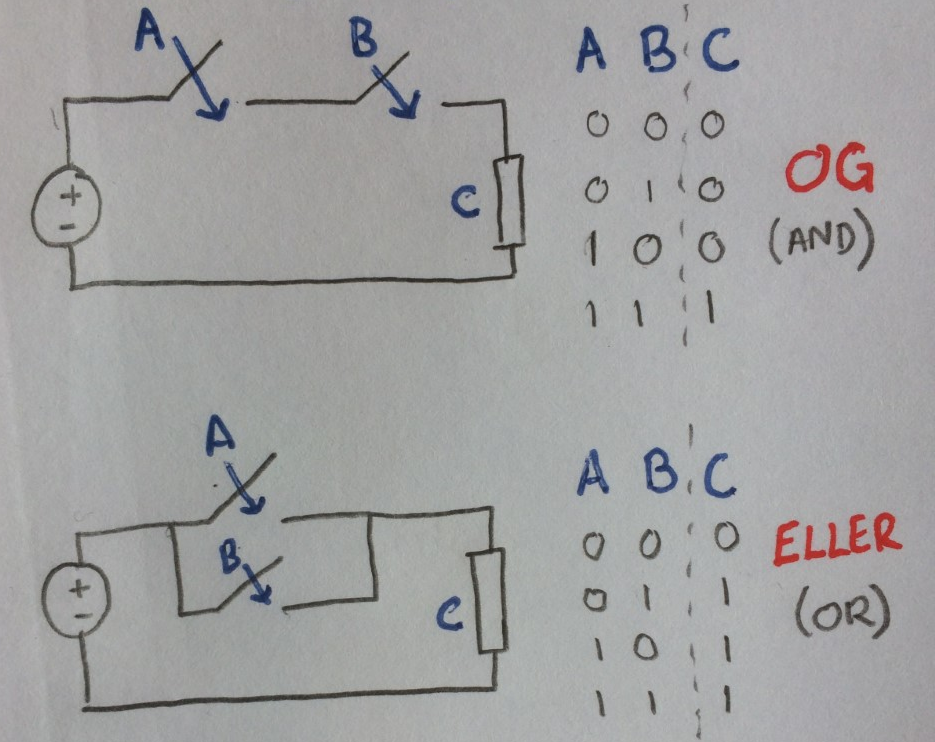
\includegraphics[width=200pt]{01_5.png}{\centering}

  \section{Oppgåve 6}
    \subsection{a)}
      Den spesielle distributative eigenskapen (+ er distributativ over $\cdot$):
      \begin{equation}
        A + \bar{A}B = (\bar{A} + A) \cdot (A + B)
      \end{equation}
      $(\bar{x} + x)$ er ein tautologi, den er alltid sann
      \begin{equation}
        A + \bar{A}B = 1 \cdot (A + B)
      \end{equation}
      derfor vert
      \begin{equation}
        A + \bar{A}B = A + B
      \end{equation}
      Dette kan vi også sjå ut ifrå sanningstabellen:

      \begin{center}
        \begin{tabular}{ |c|c|c|c| }
          \hline
          $A$ & $B$ & $A+\bar{A}B$  & $A+B$ \\
          \hline
          $0$ & $0$ & $0+(1\cdot0)=0$ & $(0+0)=0$ \\
          \hline
          $0$ & $1$ & $0+(1\cdot1)=1$ & $(0+1)=1$ \\
          \hline
          $1$ & $0$ & $1+(0\cdot0)=1$ & $(1+0)=1$ \\
          \hline
          $1$ & $1$ & $1+(0\cdot1)=1$ & $(1+1)=1$ \\
          \hline
        \end{tabular}
      \end{center}

    \newpage

    \subsection{b)}
      Om vi teikner opp sanningstabellen ser vi at $\overline{ABC}=\bar{A}+\bar{B}+\bar{C}$:
      \begin{center}
        \begin{tabular}{ |c|c|c|c|c| }
          \hline
          &&&& \\
          $A$ & $B$ & $C$ & $\overline{ABC}$  & $\bar{A}+\bar{B}+\bar{C}$ \\
          \hline
          $0$ & $0$ & $0$ & $\neg(0\cdot0\cdot0)=1$ & $1+1+1=1$ \\
          \hline
          $0$ & $0$ & $1$ & $\neg(0\cdot0\cdot1)=1$ & $1+1+0=1$ \\
          \hline
          $0$ & $1$ & $0$ & $\neg(0\cdot1\cdot0)=1$ & $1+0+1=1$ \\
          \hline
          $0$ & $1$ & $1$ & $\neg(0\cdot1\cdot1)=1$ & $1+0+0=1$ \\
          \hline
          $1$ & $0$ & $0$ & $\neg(1\cdot0\cdot0)=1$ & $0+1+1=1$ \\
          \hline
          $1$ & $0$ & $1$ & $\neg(1\cdot0\cdot1)=1$ & $0+1+0=1$ \\
          \hline
          $1$ & $1$ & $0$ & $\neg(1\cdot1\cdot0)=1$ & $0+0+1=1$ \\
          \hline
          $1$ & $1$ & $1$ & $\neg(1\cdot1\cdot1)=0$ & $0+0+0=0$ \\
          \hline
        \end{tabular}
      \end{center}

  \section{Oppgåve 7}
    \begin{equation}
      A(B+C)=AB+AC
    \end{equation}
    Vi finner den duale forma ved å bytte $+$ og $\cdot$
    \begin{equation}
      A+(BC)=(A+B)\cdot(A+C)
    \end{equation}
  
  \section{Oppgåve 8}
    \subsection{a)}
      Sidan $\cdot$ er distributativ over $+$ er
      \begin{equation}
        AC+\bar{B}C=C(A+\bar{B})
      \end{equation}

    \subsection{b)}
      \begin{equation}
        A\bar{B}\bar{C} + AB\bar{C}
      \end{equation}
      $\cdot$ er distributativ over $+$
      \begin{equation}
        A\bar{C}(B+\bar{B})
      \end{equation}
      Tautologi ($x+\bar{x}=1$):
      \begin{equation}
        A\bar{C}
      \end{equation}
    
  \section{Oppgåve 9}
    Setter opp funksjonstabell for $F(x,y,z)=xy+x\bar{y}+\bar{y}z$
    \begin{center}
      \begin{tabular}{ |c|c|c|c| }
        \hline
        &&& \\
        $x$ & $y$ & $z$ & $F(x,y,z)$ \\
        \hline
        $0$ & $0$ & $0$ & $(0\cdot0) + (0\cdot1) + (1\cdot0)=0+0+0=0$ \\
        \hline
        $0$ & $0$ & $1$ & $(0\cdot0) + (0\cdot1) + (1\cdot1)=0+0+1=1$ \\
        \hline
        $0$ & $1$ & $0$ & $(0\cdot1) + (0\cdot0) + (0\cdot0)=0+0+0=0$ \\
        \hline
        $0$ & $1$ & $1$ & $(0\cdot1) + (0\cdot0) + (0\cdot1)=0+0+0=0$ \\
        \hline
        $1$ & $0$ & $0$ & $(1\cdot0) + (1\cdot1) + (1\cdot0)=0+1+0=1$ \\
        \hline
        $1$ & $0$ & $1$ & $(1\cdot0) + (1\cdot1) + (1\cdot1)=0+1+1=1$ \\
        \hline
        $1$ & $1$ & $0$ & $(1\cdot1) + (1\cdot0) + (0\cdot0)=1+0+0=1$ \\
        \hline
        $1$ & $1$ & $1$ & $(1\cdot1) + (1\cdot0) + (0\cdot1)=1+0+0=1$ \\
        \hline
      \end{tabular}
    \end{center}

\end{document}
